\documentclass[10pt,hidelinks]{article}
\usepackage[letterpaper, hmargin=0.75in, vmargin=0.75in]{geometry}
\usepackage{graphicx}
\usepackage[hyphens]{url}
\usepackage{hyperref}
\usepackage{listings}
\usepackage{pgf}
\usepackage{fontspec}
\setmonofont{Cousine}[Scale=MatchLowercase]
\usepackage{syntax}
\usepackage{hyphenat}
\usepackage{tikz}
\usetikzlibrary{arrows,automata,shapes}
\tikzstyle{block} = [rectangle, draw, fill=blue!20, 
    text width=5em, text centered, rounded corners, minimum height=2em]
\tikzstyle{bt} = [rectangle, draw, fill=blue!20, 
    text width=4em, text centered, rounded corners, minimum height=2em]


\parindent 0in
\parskip 1.5ex


\lstset{ %
language=Java,
basicstyle=\ttfamily\scriptsize,commentstyle=\scriptsize\itshape,showstringspaces=false,breaklines=true}


\begin{document}

\title{
ECE453/CS447/SE465 \\
Software Testing, Quality Assurance, and Maintenance\\
Assignment 2, version 1.1}
\author{Patrick Lam \\
{Release Date:  February 4, 2019} \\
}
\renewcommand{\today}{}
\maketitle

\begin{center}

{\bf Due:  11:59 PM, Monday, February 25, 2019} \\
{\bf Submit: via git.uwaterloo.ca }\\
\end{center}

\section*{Getting set up}
We will create a copy of the starter repo for you in your {\tt git.uwaterloo.ca} account. You need to log in to {\tt git.uwaterloo.ca} for that to work. There is a Vagrant VM description,
but you shouldn't need it.

Tools used: python (sort of optional); g++/make (very optional); Selenium (required).

\section*{Submission summary}
Here's what you need to submit in your fork of the repo. Be sure to commit
and {\bf push} your changes back to {\tt git.uwaterloo.ca}.
\begin{enumerate}
\item in directory {\tt q1}, either file {\tt testcases.txt} or {\tt testcases.pdf}, which includes your test cases and the minimized test case and explanation; and, in directory {\tt shared/selenium/src/test/java/se465}, file {\tt CalcSuite.java} containing your test cases;
\item in directory {\tt shared/selenium/src/test/java/se465}, files {\tt CalculatorPageObject.java}, {\tt OriginalCalculatorPageObject.java}, {\tt FrancaisCalculatorPageObject.java}, along with files {\tt RefactoredCalcSuite.java} and {\tt FrancaisCalcSuite.java}.
\item in directory {\tt q3}, file {\tt fsm.pdf} as described in the question;
\item in directory {\tt q4}, your modified {\tt generate.py} file (unless you've mailed me to tell me that you're not using Python);
\item in directory {\tt q5}, file {\tt mutants.pdf} as described in the question;
\end{enumerate}
You may choose to move files into the {\tt shared} subdirectory if you want to access them in Vagrant. We'll mark submissions either in the original place or under {\tt shared}.
 
 \begin{center}
 \begin{tabular}{c|cc}
 Question   &  TA in Charge \\ \hline
1 & Parsa \\
2 & Michael \\
3 & Jason \\
4 & Meet \\
5 & Jason \\
 \end{tabular}
 \end{center}

 \newpage
\section*{Question 1 (7.5 points): More Selenium}

In your repository, you will find a JavaScript application at {\tt
  shared/calc/index.html}. I wrote this application (or at least
ported it from the Internet). It uses a Pratt parser to parse a simple expression language and evaluate the given expression.

Here is a grammar for this application. The \verb+^+ operator is supposed to denote
exponentiation.

\begin{center}
\begin{minipage}{3in}
\begin{grammar}
  <expr> ::= number 
         \alt `-' <expr>
         \alt `+' <expr>
         \alt  <expr> `+' <expr> \alt  <expr> `-' <expr>
         \alt  <expr> `*' <expr> \alt  <expr> `/' <expr>
         \alt  <expr> `\verb+^+' <expr>
         \alt `(' <expr> `)'
         
  <number> ::= [`0' - `9']$^+$
\end{grammar}
\end{minipage}
\end{center}

Your task is to manually (or otherwise) generate a set of test cases
for this application and to use Selenium to automate these test
cases. You shouldn't need to look at the application source
code, but you do need to look at the HTML of {\tt shared/calc/index.html}.

In your test suite, I recommend setting {\tt baseUrl} to one of:
\begin{itemize}
\item \verb!baseUrl = "file://" + System.getProperty("user.dir") + "/../calc/index.html";!
\item \verb!baseUrl = "https://patricklam.ca/files/calc.html";!
\end{itemize}

Specifically:

\begin{itemize}
\item (2 points) Generate 10 test cases for the application. Specify the input along with the actual and expected output. Some of the inputs must be valid strings for the application, while others must be invalid. Be sure to choose interesting test cases.

\item (3 points) The following test case exposes a bug in the application:

\begin{verbatim}
  2+(8*3/4)^4*(1+3+5)*2-4*(3/2)+9*3
\end{verbatim}

Minimize this test case. That is, produce a minimal-length subset of this test case---not necessarily using contiguous characters---which shows the same error. Explain the cause of the bug as well as the expected output.

\item (2.5 points) Use Selenium to automate your 10 test cases. In the {\tt shared/selenium} directory in your repo, you will find a {\tt SeleniumExample}. You can run tests from this example using the command:

\begin{verbatim}
mvn test "-Dtest=se465.SeleniumExample#test*" -Dwebdriver.base.url=http://www.google.com
\end{verbatim}

Your test suite should be called {\tt se465.CalcSuite} and we should be able to run your tests with this command:

\begin{verbatim}
mvn test "-Dtest=se465.CalcSuite#test*"
\end{verbatim}

We will check that your tests exercise the functionality that you specified in the first part.
Assert on all fields on the calculator page.
{\bf HINT:} You can't get the text from an input element with {\tt getText()}. See instead
\url{http://www.w3schools.com/jsref/prop_text_value.asp}.

Useful reference:

\url{https://seleniumhq.github.io/selenium/docs/api/java/org/openqa/selenium/WebElement.html}

%\item (5 bonus points) Fix a bug in the application (submit a diff).
\end{itemize}

Note: You are allowed to modify the application to add observability.

%fuzz these cases?

\section*{Question 2 (20 points): Page Objects}

Recall the Page Object design pattern from Lecture 9. Your task is to create Page Objects for the JavaScript calculator. This will allow your tests to generalize to {\tt francais.html} (and even
{\tt eval.html}, though we won't use that).

\begin{itemize}
\item (10 points) In this part, we'll create page objects. Create a generic Page Object interface {\tt se465.CalculatorPage}, along with an implementation {\tt se465.OriginalCalculatorPage}, which encapsulates the UI elements on the {\tt index.html} page. (I created the implementation first and then reverse-engineered the interface). These objects should allow you to access the controls that your tests from Question 4 need. Also, create an additional Page Object {\tt se465.FrancaisCalculatorPage} which implements the same interface but which works with {\tt francais.html}. 
  \item (10 points) Copy {\tt se465.CalcSuite} to {\tt se465.RefactoredCalcSuite}. Modify the refactored suite to use both of the page objects that you created for the first part; you should have two tests in the refactored suite for each test in the original suite. It's OK for your English and French tests to essentially be the same except for the choice of the WebDriver, or you could be more clever. (This could be done via JUnit Parameters, but we haven't talked about that.)
\end{itemize}

References for this question:

\url{http://www.seleniumhq.org/docs/06_test_design_considerations.jsp#chapter06-reference}\footnote{use a {\tt WebDriver} rather than a {\tt Selenium} object as in the example.}
\\
\url{https://martinfowler.com/bliki/PageObject.html}

\section*{Question 3 (7.5 points): FSM-Based Testing}
Consider the following FSM for the authentication part of a web app.
(inspired by \url{https://css-tricks.com/finite-state-machines-with-react/})

\begin{center}
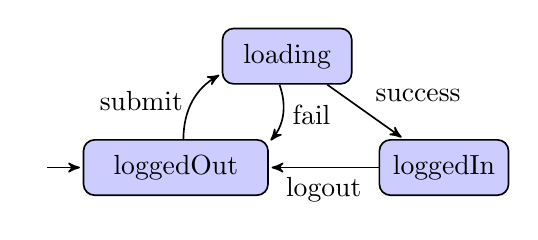
\begin{tikzpicture}[->,>=stealth',shorten >=1pt,auto,node distance=2cm,
                    semithick,initial text=]
  \node[initial,bt, text width=6em]   (1)                     {loggedOut};
  \node[bt]          (2) [above right of=1]  {loading};
  \node[bt]           (3) [right of=1,xshift=4em]  {loggedIn};

  \path (1) edge [bend left] node[left] {submit} (2)
  (2) edge [bend left] node[right] {fail} (1)
  (2) edge node {success} (3)
  (3) edge node {logout} (1);
\end{tikzpicture}
\end{center}

(2.5 points) Write out a single sequence of steps (i.e. one test case)
that achieves Complete Round Trip Coverage on this FSM, including
necessary context. For example, one of your steps could be ``Log out
of the web application''.

(5 points) A good authentication system must have anti-brute-forcing
provisions. A brute-forcing attack on this system would repeatedly try
passwords for a user until finding one that works. Describe briefly a
fix to the implementation that would prevent the attack. Does my FSM
still describe your fixed system? Write down why or why not; i.e. are
my nodes and edges still appropriate? If not, provide a modified FSM
that does.

(0 points) Think about how just looking at a model might not tell you
how to construct a test case for the brute-forcing attack.

\section*{Question 4 (10 points): Random Testcase Generation}

Your task is to write code to randomly generate valid iCalendar {\tt
  .ics} files. You can find the specification at

\begin{center}
  \url{https://tools.ietf.org/html/rfc5545}
\end{center}
Although you will be marked against the full specification, following
the description of the subset here will suffice.

\begin{itemize}
  \item an {\tt ics} file starts with a {\tt BEGIN:VCALENDAR} line and
    ends with an {\tt END:VCALENDAR} line. It must also contain a {\tt
      VERSION} and {\tt PRODID} line. (The provided code generates
    these for you.)
  \item your {\tt ics} file should contain a sequence of events.  Each
    event starts with {\tt BEGIN:VEVENT} and ends with {\tt
      END:VEVENT} and contains a set of components.  Each event must
    contain UID, DTSTAMP and DTSTART components. Valid iCalendar
    events may contain other components, and we'll be checking that
    your events do contain some other components.
  \item the {\tt UID} must be a string that is unique per-event;
  \item the {\tt DTSTAMP} and {\tt DTSTART} components must contain dates/times, which are
    yyyymmddThhmmssZ, with T and Z literal and dates/times as appropriate.
  \item other valid components include {\tt LOCATION}, {\tt SUMMARY}, and {\tt DTEND}.
\end{itemize}

You will find a {\tt generate.py} file with skeleton code in the {\tt q1} directory of your repo.
You can also find a number of sample {\tt ics} files in the {\tt shared/icalendarlib} directory.
I can run the Python file with {\tt python generate.py} at a prompt.

You are not required to use the skeleton {\tt generate.py}; if you choose to write your own
generator, email me (Patrick) to let me know. The path of least resistance is
using the provided skeleton. You just need to add new rules to the CFG at the end of {\tt generate.py}
and new special productions to {\tt generate\_special\_production}. (My solution adds 4
special productions and 9 {\tt add\_prod} lines to the CFG; you don't really need to know
Python to solve this problem, just pattern-match against what's there already.)

\paragraph{Marking scheme.} We will mark this by running your code 20 times to generate
          {\tt ics} files. We then check that the files are different and that they include more
          than zero events and also more than zero optional components. Finally, we'll check
          your generated files for validity against the iCal spec using an automated tool.

\paragraph{Bonus (0 marks).} Can you create valid {\tt ics} files that break the app in {\tt shared/icalendarlib}? (I can't.)

%In the {\tt shared/icalendarlib} directory, you will find an implementation of
%an iCalendar {\tt ics} file parser, which can (perhaps) validate your generated files.
% https://icalendar.org/validator.html
          
You can find links to more sample {\tt ics} files here:\\
\url{http://apple.stackexchange.com/questions/125338/calendar-ical-ics-format}

\section*{Question 5 (10 points): Mutation Testing} 

Consider the following implementation of the cycle-finding algorithm\footnote{A more verbose implementation: \url{https://en.wikipedia.org/wiki/Cycle_detection}.}. (We've included the complete implementation from there in the skeleton at {\tt q5/cycle-finder.c}, including a test harness.) In your {\tt q5/mutants.pdf} file, propose two non-stillborn and non-equivalent mutants of this function. Clearly indicate where you've mutated the ground string. Write down test inputs which strongly kill these mutants (syntax doesn't matter) and the expected output of your test cases on the original code and on the mutant.

\vspace*{-1em}
\begin{lstlisting}
typedef struct node_s {
        void *data;
        struct node_s *next;
} NODE;

int list_has_cycle(NODE *list)
{
        NODE *fast=list;
        while(1) {
                if(!(fast=fast->next)) return 0;
                if(fast==list) return 1;
                if(!(fast=fast->next)) return 0;
                if(fast==list) return 1;
                list=list->next;
        }
        return 0;
}
\end{lstlisting}



\end{document}
